\documentclass[12pt]{article}
\usepackage[a4paper, margin=.30in]{geometry}
\usepackage{graphicx ,
            wrapfig,
            xcolor, 
            enumerate,
            amsmath,fontenc, mhchem  ,tcolorbox 
            }

\newcommand\headerMe[2]{\noindent{}#1\hfill#2}
\renewcommand{\thesection}{\Roman{section}}

\author{Zakaria HAOUZAN}
\date{\today}

\begin{document}
% headers --------------
\headerMe{Matière : Physique-Chimie}{Professeur : Zakaria HAOUZAN}\\
\headerMe{Unité : Travail Mécanique et Energie }{Établissement : Lycée SKHOR qualifiant}\\
\headerMe{Niveau : 1BAC-SM-X}{Heure : 1H}\\

% ------Content ________
\begin{center}

  \Large{Leçon $N^{\circ} 8 $: \color{red}Evolution  de la chimie organique. }
\end{center}

%\begin{wrapfigure}[10]{r}{0.5\textwidth}
%    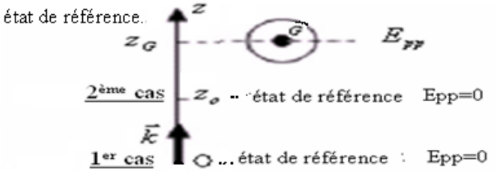
\includegraphics[width=0.5\textwidth]{./img/img00.png}
%\end{wrapfigure}


%\begin{tcolorbox}[colback=pink!10!white,
                  %colframe=blue!15!gray,
                  %title=Application -1- :
                 %]


  %\begin{wrapfigure}[10]{r}{0.3\textwidth}
  %\vspace{-2cm}
    %\includegraphics[width=0.3\textwidth]{./img/Mode_opératoire_dosage:.png}
%\end{wrapfigure}


\section{Chimie organique et ses champs :}
  \subsection{ Définition de la chimie organique: }
  La chimie organique est la chimie des composés carbonés d'origine naturels ou synthétiques.
  \subsection{Ressources naturelles : }
Les ressources naturelles de la chimie organique sont : 
  \begin{itemize}
      \item La photosynthèse: Sous l'action de la lumière, les végétaux transforment le "carbone minéral" en "carbone organique" (glucides).
        \\exemple : synthèse du glucose $\ce{6{CO_2}_{(g)}+ 6{H_2O}_{(l)} -> {C_6H_{12}O_6}_{(aq)} + 6O_2  }$
        \item Les synthèses biochimiques:
Il s'agit des transformations chimiques effectuées par les cellules des êtres vivants à partir des"aliments"conduisant
à la formation de composés organiques.
\item Les hydrocarbures fossils:
Les hydrocarbures fossiles (pétrole et gaz naturel) proviennent de la décomposition de matières organiques.

  \end{itemize}
  \begin{wrapfigure}[10]{r}{0.1\textwidth}
  %\vspace{-2cm}
    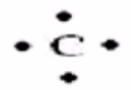
\includegraphics[width=0.1\textwidth]{./img/carbone_foem.png}
\end{wrapfigure}

  \section{ L'élément de base de la chimie organique : (Le Carbone)}
  L'atome de carbone a pour numéro atomique Z=6 , sa structure électronique est : $(K)^2(L)^4$.

Il a quatre électrons dans la couche externe donc quatre électrons de valence, on dit que l'atome de carbone est
tétravalent.
Le modèle de Louis pour l'atome de carbone est :


Dans tous les composés organiques l'atome de carbone ne participe que par quatre liaisons avec les atomes voisins.
  \begin{center}
    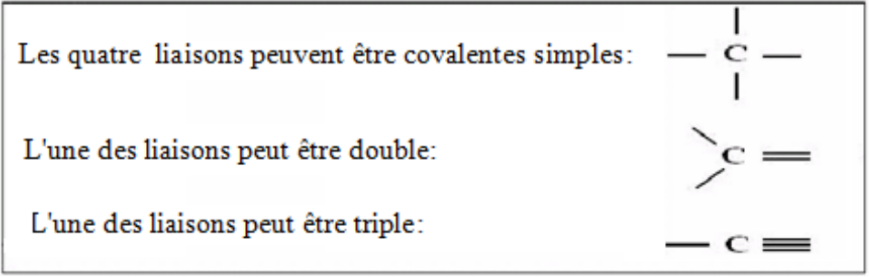
\includegraphics[width=0.5\textwidth]{./img/four_carbone.png}
    \end{center}
    \section{Importance de la chimie organique : }
    La chimie organique est considérée comme la base de l'économie mondiale , car elle fournit la matière première à
tous les autres domaines.

On distingue les secteurs de la chimie organique selon les produits formés:

  - La chimie lourde: Elle assure la fabrication des matières plastiques et du caoutchouc. Cette production en gros
tonnages s’effectue en peu d’étapes et à partir de matières premières facilement accessibles.

- La chimie fine :Elle produit des molécules plus complexes utilisées dans la formation et la fabrication de produits
pharmaceutiques ou parachimiques.
\end{document}

